\section{Strategy}
\label{Strategy}
We find it interesting to research the design of smarter players, who take into account board characteristics when deciding which marble to place or which sub-board to rotate.
There are two players in the game. Each player has a flag if he is employing a specific strategy or plays randomly. 
To compare two players we use a monte carlo style method: We execute a number of playthroughs until one of the final states is achieved(draw or a player wins).
From these playthroughs we gather the execution time, the number of transitions taken and the result of the game.

\vspace{6pt}
\subsection{strategy2}

A strategy2 player tries to do two types of moves:
\begin{itemize}
\item Try to extend the longest consecutive row of marbles of its color.
\item Place a marble in a center position
\end{itemize}

In order to make decisions it first tries to look for a row of 4 marbles and places one marble at either possible end. If this is not available it looks for a row of 3. This patern repeats till the length of the row is 1.
If it can not find a free Space adjacent to a marble of its own, then it will try to occupy a Space in the center of a block.
If none of the strategy rules can be matched, the system will fall back by placing a marble in a random empty Space.

Rules and control programs to model the strategy are placed in the "strategy" folder/ package.

\begin{figure}[!h]
  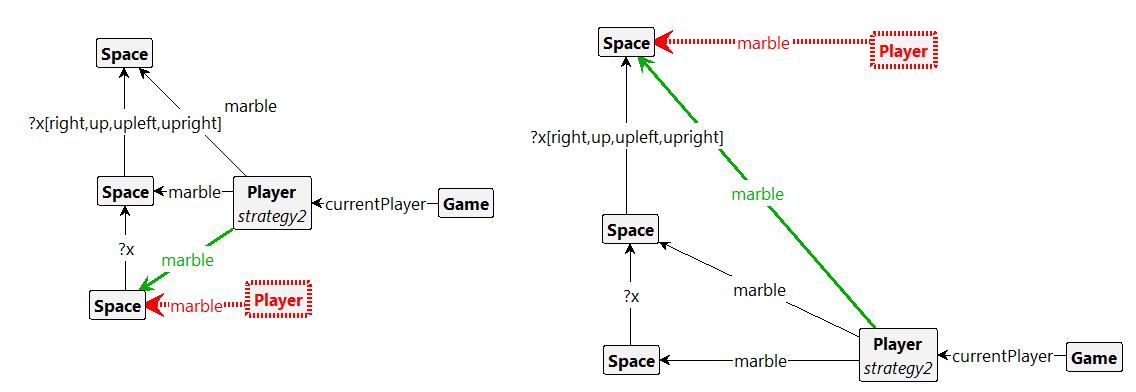
\includegraphics[scale=0.5,clip]{Images/twocombined.png}
  \caption{Types overview}
  \label{fig:twocombined}
\end{figure}

\subsubsection{The rules}

A player has won if it has 5 marbles in a row. Therefore the first situation we want to cover is when a player already has 4 marbles in a row, and an adjacent space is free.
Since the directions are one-way we get two rules for this situation: one for placing a marble at the left end of the row (add2fourLeft) and one to add to the right of the row (add2fourRight).
Similar rules have been made for rows of length three, two and one.\\
These "rows'" can of course be in 4 different directions. To prevent a blowup in the number of rules we chose to use a wildcart for the direction edges, that have to match with "up", "down", "downleft" or "downright".
This does make the analysis somewhat slower, since these rules are harder to match. However we feel it is justified because otherwise we would need 4 times the 4 rules to model each direction.

If there is no existing row to extend, the strategy2 player tries to place a marble in the center space of a block. This can easily be done by matching on the "place5" flag that is already present on the board for supporting the rotations. This is done in the "midBlock" rule.

If the center spaces are also occupied then there are no strategy rules to match. Then the control program manages that it falls back to (one of) the remaining available spaces.

\subsubsection{Control Program}

The strategy2 has its own control program in the strategy package to enforce the order in which the rules are matched.
The function "pm" (short for place marble) first tries to match one of the rules to extend 4-in-a-row, then for 3 and so on. The last option is to try to match "midBlock" to place a marble in the center of a block.

To make sure that a player uses its appointed strategy, the "game\_progress" control program in the main package was also updated.
The "executePlace" function first tries to match strategy rules by calling the "pm" function of the strategy. If none of these rules match, either because the player has no strategy flag or because the strategy is exhausted, then it will try to match the general "placeMarble" rule.

Since the strategy2 player has no strategy for turning blocks, there are no additional rules or control programs needed for this part of the game.

\subsection{Results}
To be able to draw a conclusion about whether our strategy performs well, we want to formally evaluate its performance.
Because the game is relatively complex, it is impossible to generate the entire state space of the game, and determine the complete win rate of the naive and the smart strategies.
Therefore we have decided to perform a Monte Carlo simulation. A Monte Carlo simulation produces distributions of possible outcome values.

\vspace{6pt}

TODO

To determine the number of iterations needed to meet these requirements, we use the following formula \cite{sim-modeling}:

%n = (zα/2 S / E ) ²
